
\documentclass{article}

\usepackage{amsfonts}
\renewcommand*\familydefault{\sfdefault}

\usepackage[comma,authoryear]{natbib}
\renewcommand{\bibname}{References} % DO NOT remove or switch of 
\usepackage[hypcap=true]{caption}
\usepackage[french]{babel}
\usepackage[cmex10]{amsmath}
\usepackage{amssymb}
\usepackage{amsthm}
\newtheorem{mydef}{Definition}
\newtheorem{mytherm}{Theorem}
\usepackage{hyperref}
\usepackage{varioref}

\usepackage[T1]{fontenc}
\usepackage[ruled,linesnumbered]{algorithm2e}
\usepackage{algpseudocode}
\renewcommand{\algorithmicrequire}{\textbf{Input:}}
\renewcommand{\algorithmicensure}{\textbf{Output:}}
\usepackage[utf8]{inputenc}
\usepackage{listings}
\usepackage{xcolor}
\definecolor{codegreen}{rgb}{0,0.6,0}
\definecolor{codegray}{rgb}{0.5,0.5,0.5}
\definecolor{codepurple}{rgb}{0.58,0,0.82}
\definecolor{backcolour}{rgb}{0.95,0.95,0.92}

\lstdefinestyle{mystyle}{
    commentstyle=\color{codegreen},
    keywordstyle=\color{magenta},
    numberstyle=\tiny\color{codegray},
    stringstyle=\color{codepurple},
title=\lstname
}

\lstset{style=mystyle,breaklines=true,xleftmargin=\parindent}



\usepackage{graphicx}
\usepackage{subfigure}
\usepackage{caption}
\usepackage{lipsum}


\usepackage{multirow}
\usepackage{rotating}
\usepackage{makecell}
\usepackage{booktabs}

\usepackage{enumitem}
\newlist{abbrv}{itemize}{1}
\setlist[abbrv,1]{label=,labelwidth=1in,align=parleft,itemsep=0.1\baselineskip,leftmargin=!}




\usepackage[toc]{appendix}

\begin{document}
    
    \begin{titlepage}      
        \begin{center}
            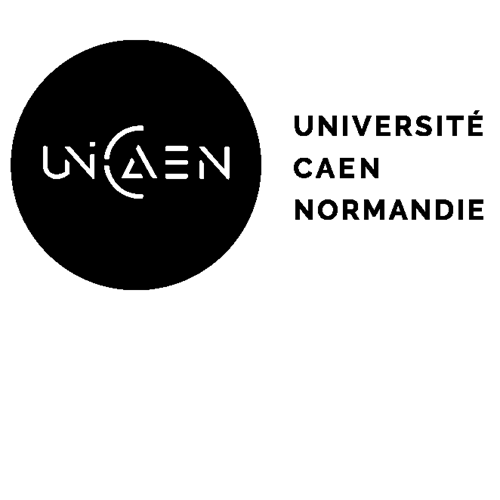
\includegraphics[width=7cm]{figures/logoUNICAEN.png}\\[0.5cm]
            {\LARGE Licence 2 Informatique\\[0.5cm]
            Groupe TP 2B}\\[1cm]

            \linespread{1.2}\huge {
            
                Simulateur de jeux de la vie
            
            }
            \linespread{1}~\\[1cm]
			%{\color{blue} \rule{\textwidth}{1pt}}
            {\Large 

                Remi Brouazin,\hspace{0.1in} Lorenzo Fanit, \hspace{0.1in} \\Yassmine Habil,\hspace{0.1in} Jody-Ange Agbohouto.
                % change end             
            }\\[1cm] 
            

            {\large 
         
                \emph{Superviseur de Projet:} CAGNIOT Emmanuel}\\[1cm] % if applicable

            \large 

            \vfill
            
            
            \today % Please update this date you can use \date{April 2020} for fixed date
        \end{center}
    \end{titlepage}
    
    
    % -------------------------------------------------------------------
    % Declaration
    % -------------------------------------------------------------------
    \newpage
    \thispagestyle{empty}
     
    \noindent

    \noindent

    
    \tableofcontents
    \listoffigures
    \listoftables

    \newpage
    
    \section{Introduction}



\subsection{Description générale du projet}
	Le jeu de la vie est un automate cellulaire inventé par le mathématicien John Horton Conway au début des années 1970. Le jeu en fait c'est comme un quadrillage avec une multitude de cases, où chaque case peut être dans deux états possibles : "vivante"  ou "morte". L'état de chaque case à un instant donné dépend de l'état de ses 8 cases voisines à l'instant précédent, selon des règles données.
\begin{enumerate}
	\item Les règles de Conway: 
 
        \begin{itemize}
            \item Une cellule morte entourée exactement de trois cellules vivantes devient vivante à la génération suivante (naissance).
            \item  Une cellule vivante entourée de deux ou trois cellules vivantes reste vivante à la génération suivante.
            \item Toute autre cellule vivante meurt à la génération suivante de surpopulation ou de sous-population.

        Le Jeu de la Vie selon les règles de Conway est le plus connu.
        \end{itemize}
	\item Le High life:
            \begin{itemize}
                \item Les règles du High Life sont similaires à celles du Jeu de la Vie de Conway, mais avec une règle supplémentaire : une cellule vivante entourée de six ou sept voisines vivantes reste vivante à la génération suivante.
                 \item Le High Life présente également divers motifs mais il peut générer des structures uniques par rapport au Jeu de la Vie de Conway en raison de cette règle supplémentaire.
            \end{itemize}
	\item Le Day \& Night:
            \begin{itemize}
                \item C'est un automate cellulaire similaire au Jeu de la Vie de Conway, mais il fonctionne dans des conditions cycliques où le nombre de cellules vivantes (noires) dans un quart de la grille doit être égal au nombre de cellules mortes (blanches).
                
            \end{itemize}
 
\end{enumerate}

En fait, il ne s'agit pas véritablement d'un jeu jeu au sens propre mais d'une sorte de simulation de l’évolution de cellule sur une surface. 

Dans un premier temps, il s'agit de réaliser une interface permettant de visualiser un tel jeu et définir différentes règles d’évolution.

Tout au long de dévéloppement du jeu, on a beaucoup utilisé un vocabulaire pratique pour décrire des facteurs dans le jeu.

\begin{itemize}
    \item La sous-population: Une cellule vivante avec moins d'un nombre défini de voisins meurt d'isolement.
    
    \item La survie: Une cellule avec un nombre défini de cellules voisines survie à la prochaine génération
    \item La sur-population: Une cellule avec un certain nombre de cellules voisines meurt de sur-population.
    \item La naissance: Une cellules morte avec un nombre défini de voisins naît 
\end{itemize}

L'evolution de la grille peut produire des schéma différents, notamment:
\begin{enumerate}
    \item Configurations stables:
    \item Les oscillateurs: Des schémas qui se répètent sur un certain nombre de générations
    \item Les vaisseaux: Des motifs qui se déplacent sur la grille
\end{enumerate}

En jouant, on peut observer les motifs se dessiner ou apparaître par rapport aux configurations pré-definis
Players can observe these patterns unfold or set initial configurations to see how they evolve over time.

Le jeu de la vie à plusieurs applications en informatique, en mathematiques et même en biologie. Il sert de modèle for etudier des systèmes complexes et pour des algos de dévéloppement.

\subsection{Description générale de la problématique}

Dans le contexte d'implémenter ce jeu, nous allons nous frotter à dans notions essentiels à maîtiser pour tout bon dévéloppeur logiciel:

\begin{enumerate}
    \item Premièrement, d'implémenter une grille 2-dimensions pour répresenter les cellules.
    Les cellules pourront être représentées soit avec des valeurs booléenes ou avec un ENUM.

    \item L'initialisation de la grille avec une configuration initiale de cellules morte comme vivantes. Cela pourra être fait aléatoirement ou en utilisant une grille définie.
    
    \item Un algorithme spécifique, appelé HashLife, avec une structure de donnée adaptée permettant de calculer rapidement l'état suivant d'une grille. En effet, lorsque le nombre de cellule est trop grand, une méthode de calcul naïve peut être extrêmement coûteuse.

    \item Appliquer une boucle pour simuler l'évolution sur toutes les génération en appliquant les règles à chaque fois en mettant à jour toujours au dernier état

    \item Faire appliquer toutes les règles pour déterminer si une cellule survie, meurt ou naît, mais faire appliquer sur l'entièreté de la grille

    \item Utiliser une GUI (Graphics user interface): Afficher la grille dans une fenêtre où les cellules peuvent être représentées par des carrés de couleur (par exemple, noir pour vivant, blanc pour mort).
 Mettre à jour l'affichage en temps réel pour montrer la progression des générations.

 \item Interaction utilisateur: Permettre à l'utilisateur d'interagir pour modifier la grille, changer les configurations initiales ou interrompre/reprendre la simulation.
Mettre en place des contrôles pour démarrer, arrêter et réinitialiser la simulation si nécessaire.

    \item Outils de programmation : Evoluer avec le de programmation imposé: JAVA avec Swing pour la partui GUI.
    
    Utiliser efficacement les structures de données et les algorithmes pour gérer les opérations de la grille et la logique de simulation.
    
    \item Test et analyse :
Tester la mise en œuvre avec différentes configurations initiales et différents ensembles de règles afin d'observer et d'analyser les comportements émergents.


\end{enumerate}



    \section{Objectifs du projet}
\label{ch:lit_rev} 

\subsection{Description plus précise de ce qu'il fallait faire} 

Dans un premier temps, il était question de développer une application informatique qui simule le jeu de la vie basé de Conway.
Pour cela il fallait un modèle du jeu simulable depuis le terminal, ensuite créer une représentation graphique de la grille et des cellules.

Pour ce faire, une étude et comprehension des règles du jeu de la vie était nécessaire.
En utilisant des concepts de programmation orientée objet pour traiter le comportement des membres du jeu. Aussi, devait être implementée la partie graphique conviviale permettant à l'utilisateur d'interagir avec la simulation.
Trouver une façon de gérer les états des cellules (vivant ou mort) selon les règles prédéfinies.
Réaliser des tests unitaires pour garantir le bon fonctionnement des classes et des méthodes.

Documentation et Rapport : Documenter le code source avec des commentaires et les contrats des differentes méthodes.
Rédiger un rapport détaillé expliquant la conception, l'implémentation, les résultats et les problèmes rencontrées

Présenter le projet de manière structurée avec des illustrations, des captures d'écran et des diagrammes explicatifs (diagrammes de classes, etc...)

\subsection{Description de travaux existants sur le même sujet}

Mise à part la publication originale du jeu par John Conway, plusieurs logiciels de simumlation du jeu de la vie ont vu le jour: 
Ces simulateurs permettent aux utilisateurs d'explorer les règles du jeu, d'observer les motifs émergents et de tester différentes configurations de cellules.
\begin{itemize}
    \item \href{https://neuralpatterns.io/}{Automates cellulaires neuraux}
    \item \href{https://www.geekpassion.fr/jeu-de-la-vie}{Jeu de la vie classique}
    \item \href{https://www.dcode.fr/jeu-de-la-vie}{Jeu de la Vie - Automate Cellulaire avec Règles} 

\end{itemize}

Aussi les Forums et Communautés en ligne de passionnés du "Jeu de la Vie". disposent de forums et sites web dédiésqui permettent aux utilisateurs de partager des créations, des astuces de programmation et des découvertes liées au jeu.

Comme indiqué précedemment en introduction, le jeu de la vie à plusieurs applications dans différents métiers:
Par exemple: 
\begin{itemize}
    \item En Physique : simulation d’écoulements, transfert de chaleur, résistance des matériaux, météorologie…
    \item En Chimie : optimisation géométrique de molécules complexes, mécanique moléculaire, dynamique moléculaire, diffusion de molécules dans des solides poreux, simulation de polymères, transitions de phase…
    \item En Biologie : modélisation de grosses molécules (ADN, protéines, etc), de leur configuration spatiale, de leurs interactions, simulation de comportements collectifs (fourmis, bactéries, etc)…
    \item En Informatique : réseaux de neurones, automates cellulaires, vie et intelligence artificielles…
    \item En Mathématiques : logique, indécidabilité, phénomènes chaotiques…
\end{itemize}








    
\section{Fonctionalites}
\subsection{Description des fonctionalités}

         Notre projet à la possibilité de simuler le jeu de la vie, selon les règles de conway, du HighLife ou du Day \& Night. 
         \begin{figure}


 \begin{center}
    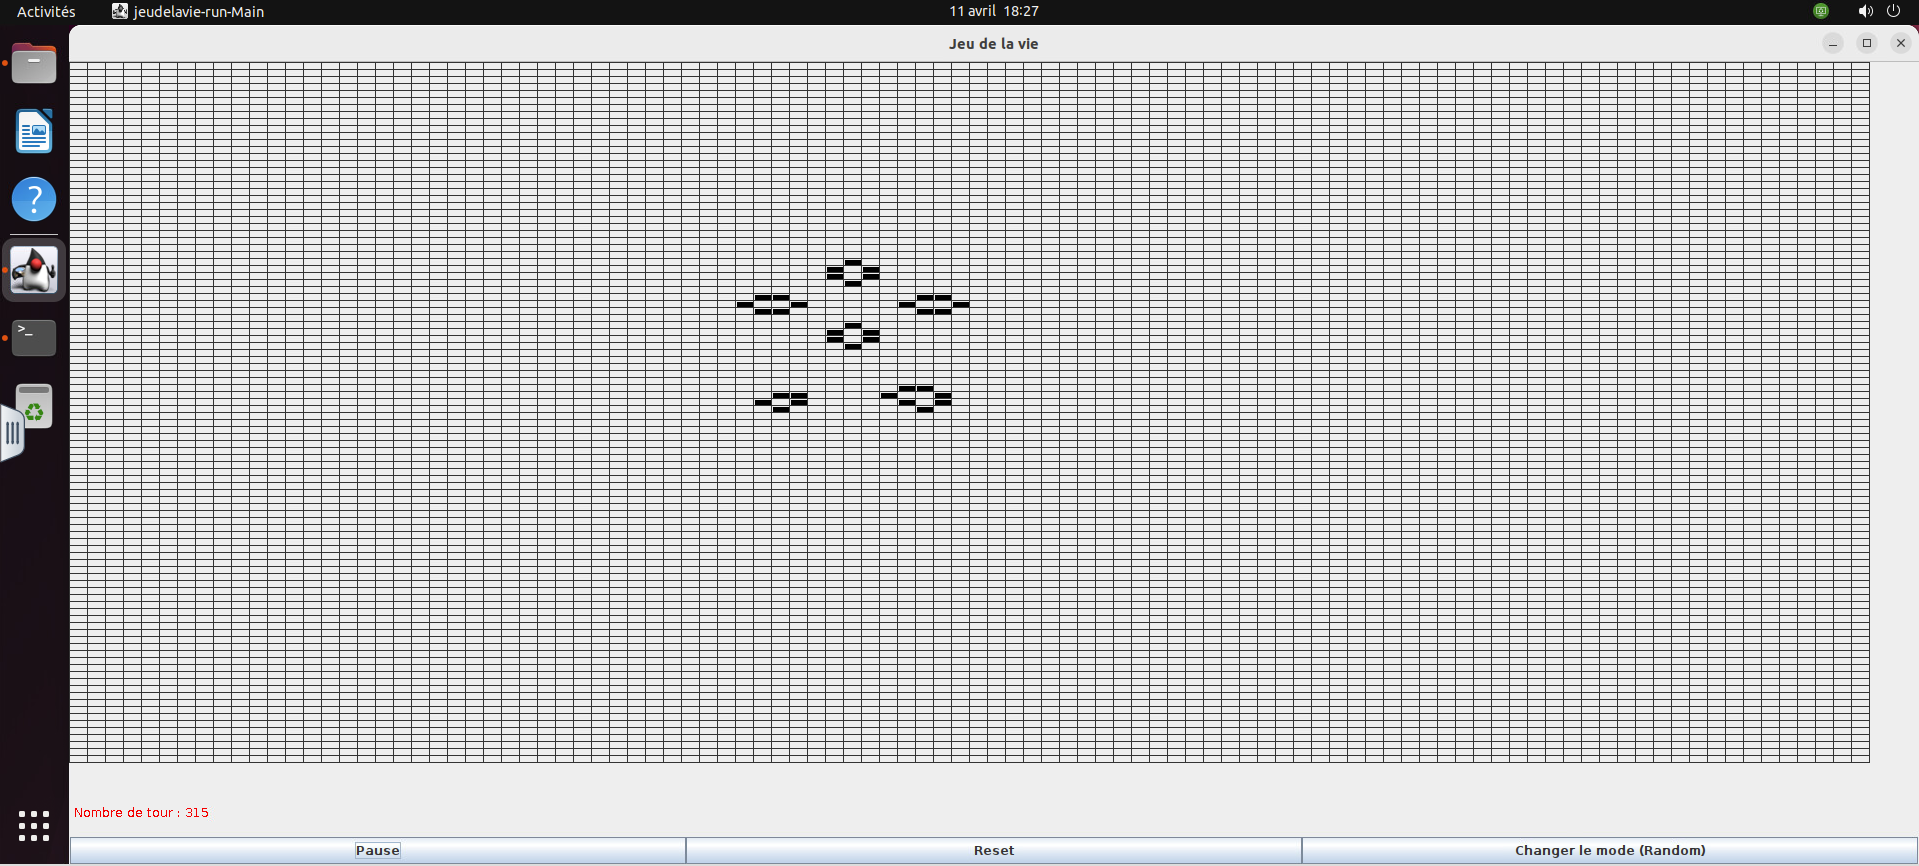
\includegraphics[width=120mm,scale=0.5]{figures/jeu.png}
    \captionof{figure}{Capture d'écran du jeu}
 \end{center}
         \end{figure}
    Avec comme cellules vivantes à la première génération, soit des cellules générés aléatoirement, importés depuis un fichier ou séléctionés sur la grille via des clicks sur l'interface graphique.
\begin{figure}
\begin{center}

    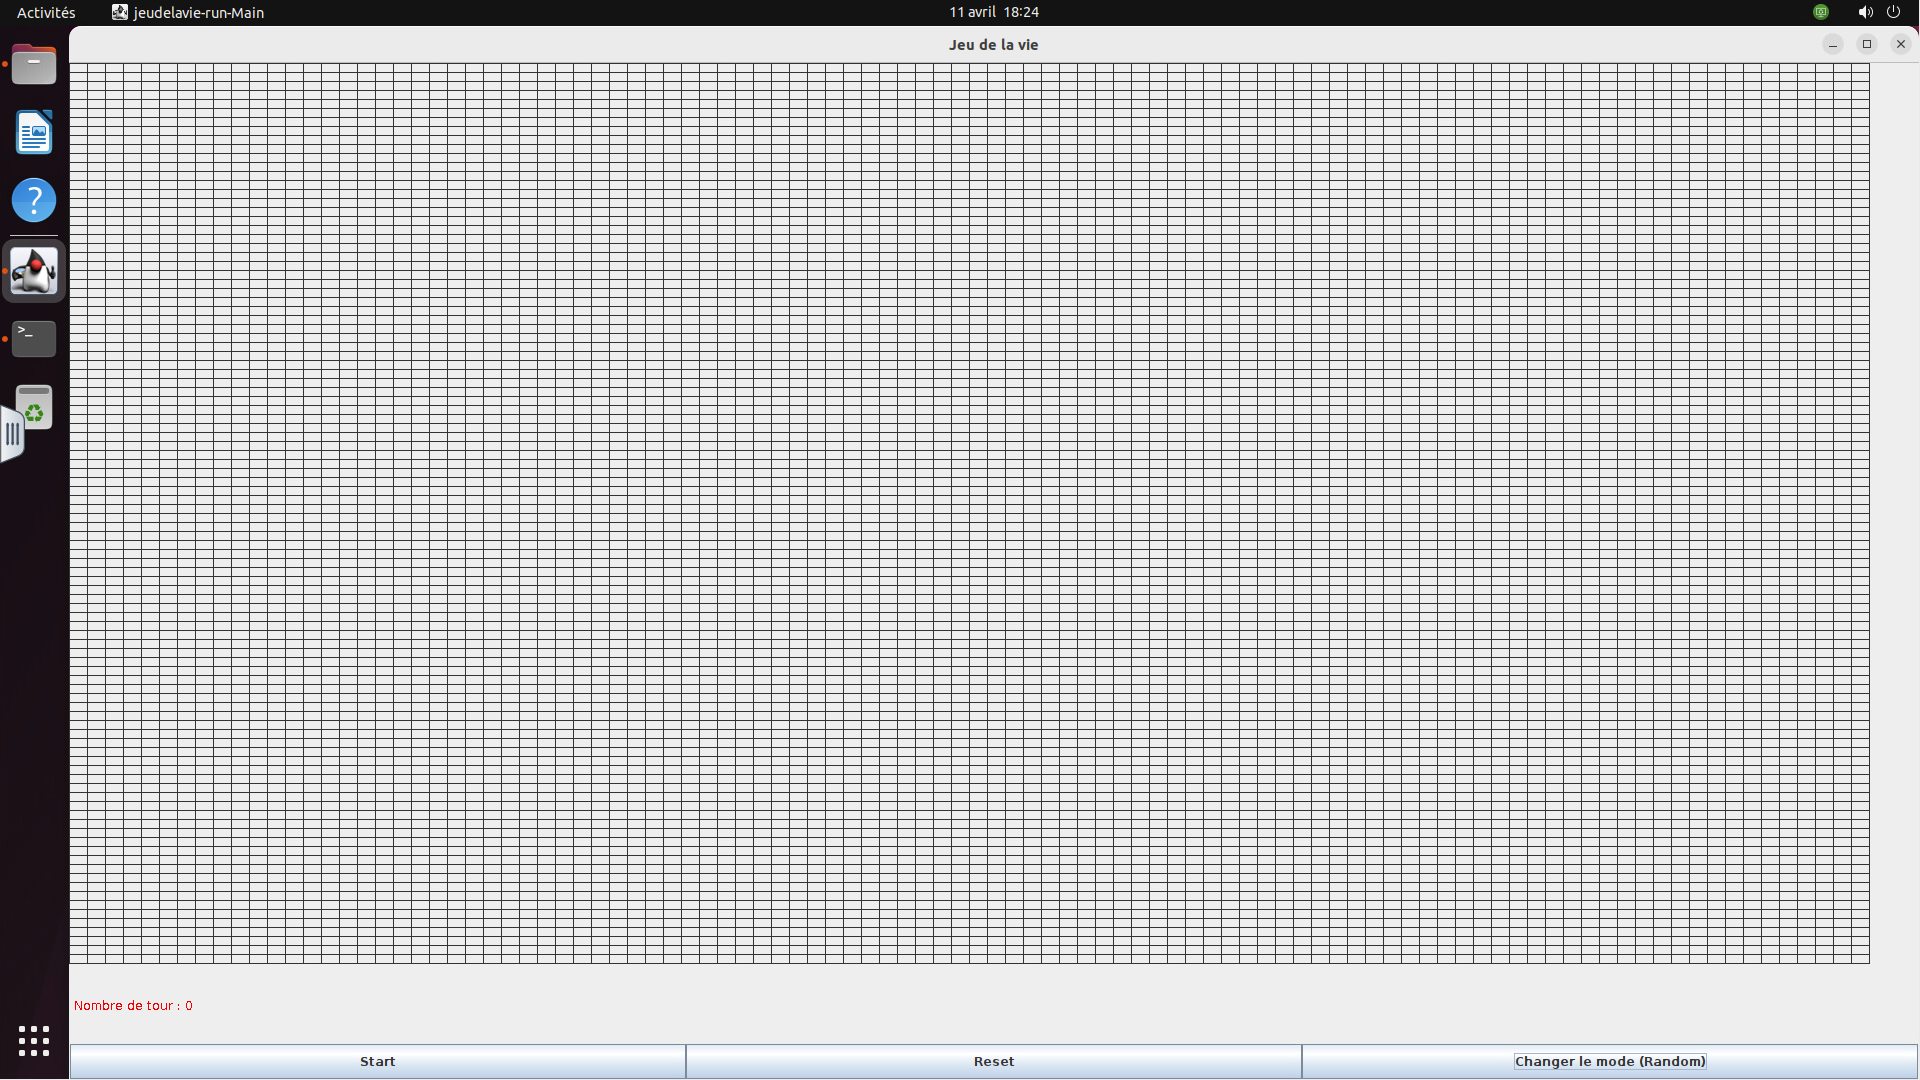
\includegraphics[width=120mm,scale=0.5]{figures/click_mode.png}
    \captionof{figure}{Mode grille cellules cliquables}

    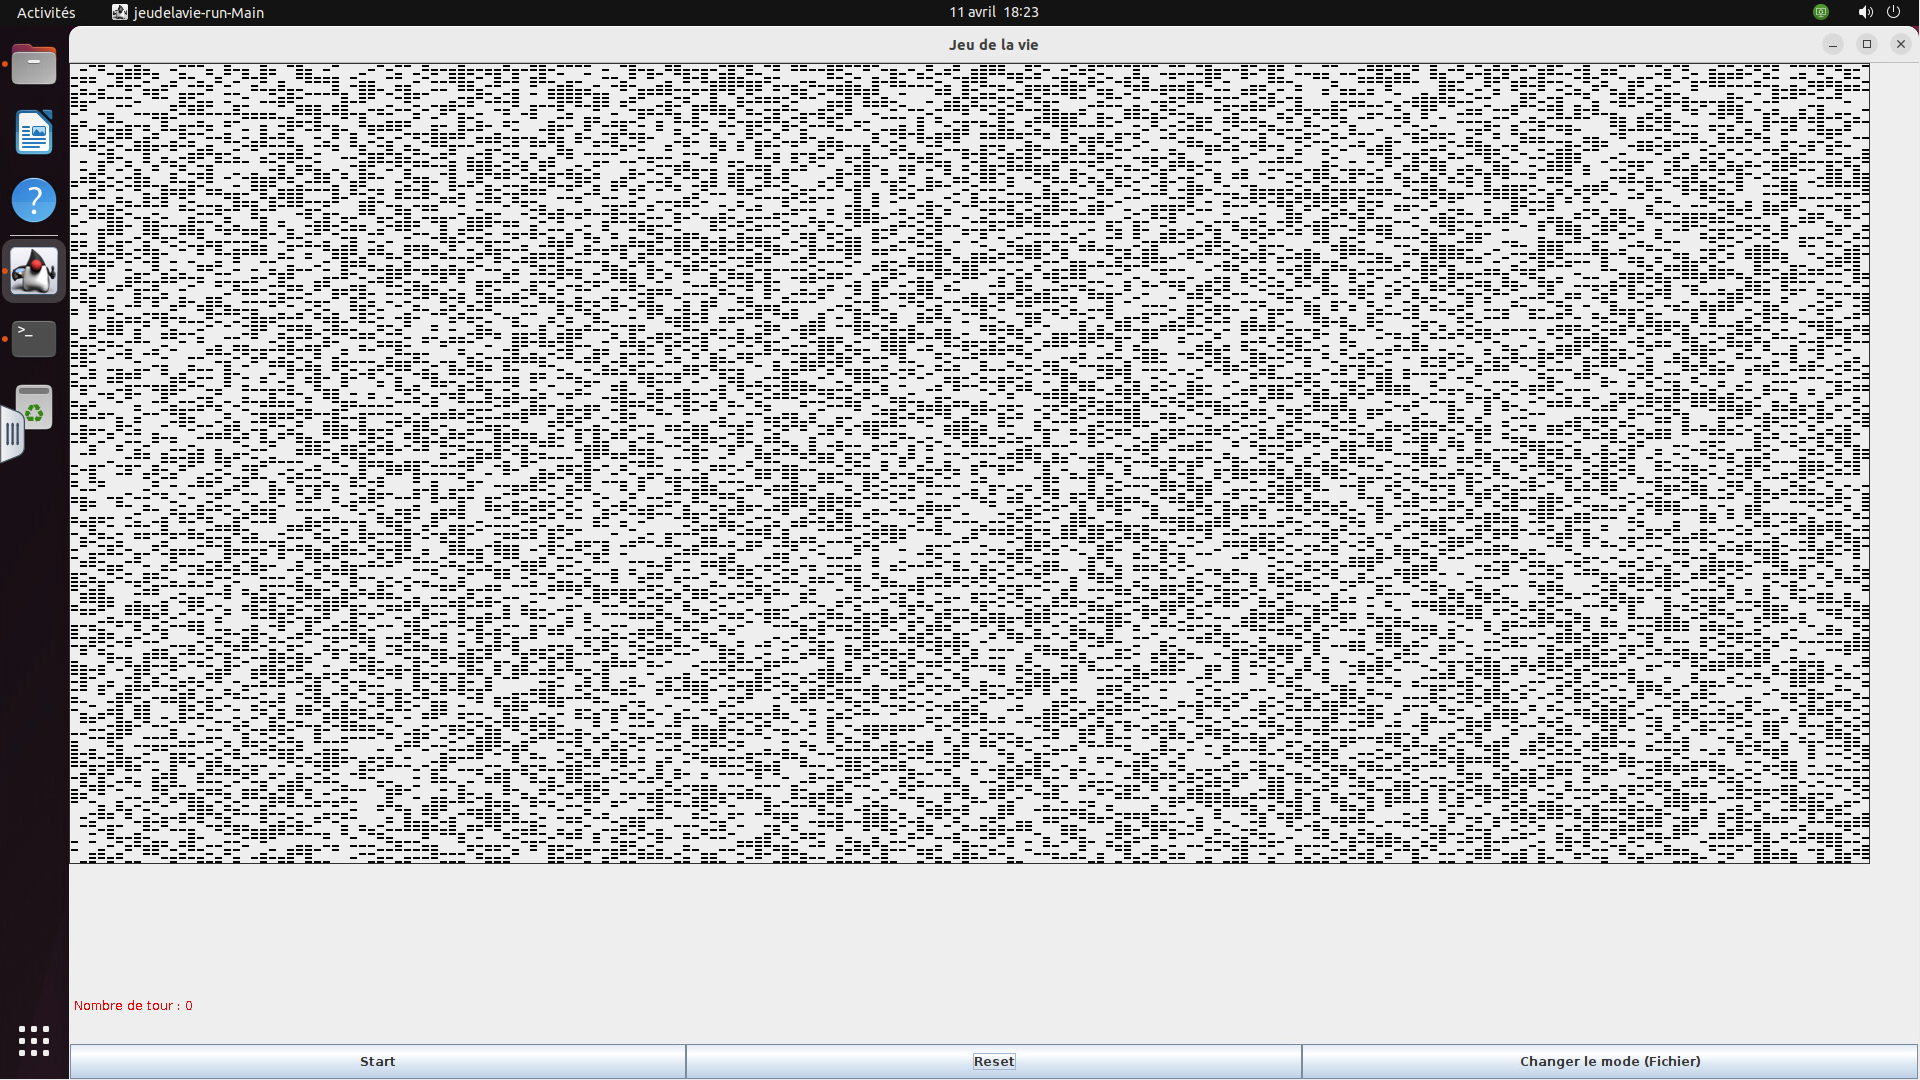
\includegraphics[width=120mm,scale=0.5]{figures/mode_random.png}
    \captionof{figure}{Génération de cellules aléatoirement sur la grille}
\end{center}
\end{figure}

    Le jeu est capable d'upscale comme de downscale, de switcher par exemple d'un affichage 100x100 à 10x10.
    \begin{figure}


\begin{center}
        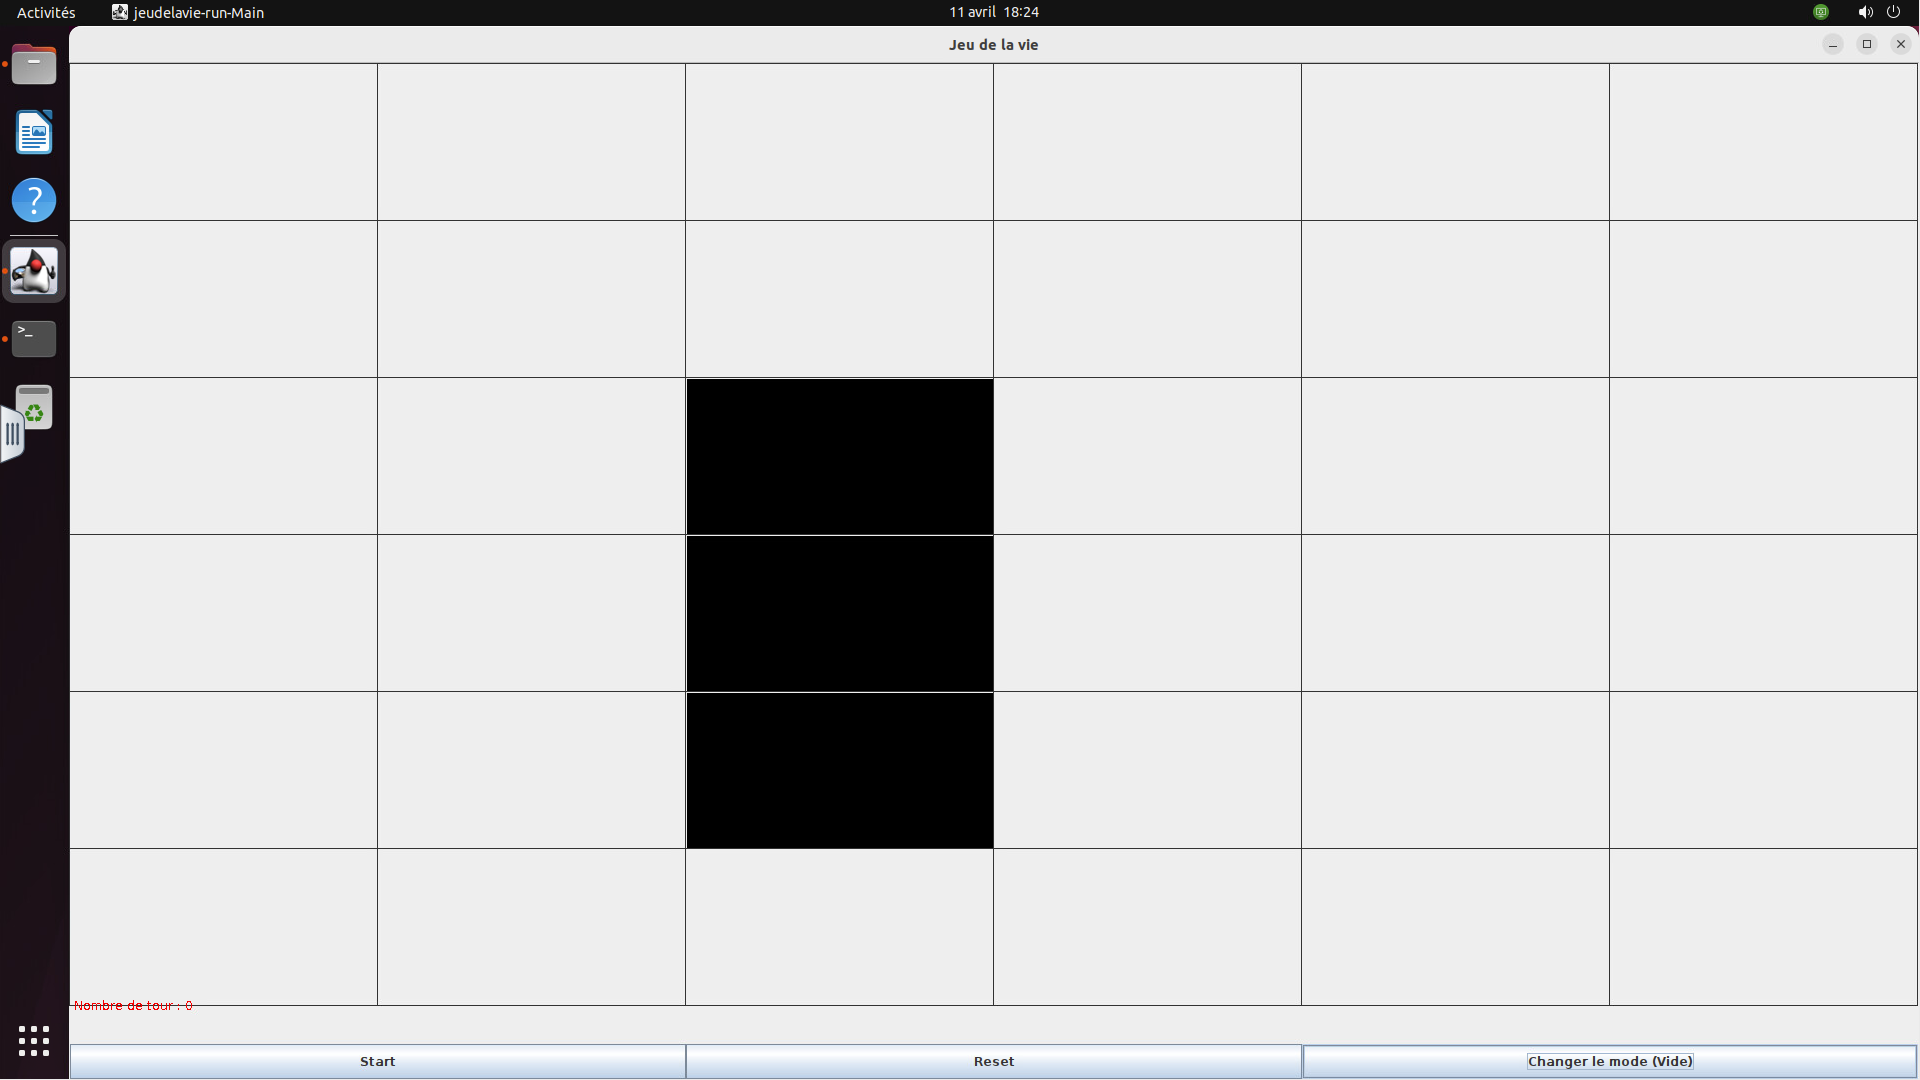
\includegraphics[width=120mm,scale=0.5]{figures/mode_file.png}
    \captionof{figure}{Mode grille depuis un fichier}
\end{center}
\end{figure}
    
    Avant le lancement de la simulation, sur l'interface graphique, 3 boutons sont visibles:

\begin{figure}

\begin{center}
    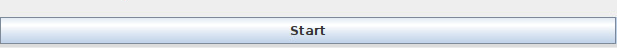
\includegraphics[width=120mm,scale=0.5]{figures/start_btn.png}
    \captionof{figure}{Bouton "Start"}
    
    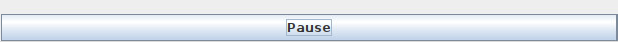
\includegraphics[width=120mm,scale=0.5]{figures/pause_btn.png}
    \captionof{figure}{Bouton "Pause"}
    
    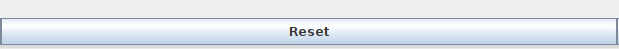
\includegraphics[width=120mm,scale=0.5]{figures/reset_btn.png}
    \captionof{figure}{Bouton "Reset"}
    
    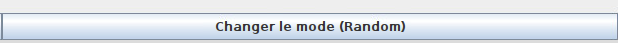
\includegraphics[width=80mm,scale=0.5]{figures/change_btn.png}
    \captionof{figure}{Bouton "Changer de grille"}
\end{center}

\end{figure}

Pour lancer le jeu, il faut cliquer sur le bouton "Start", une fois que la simulation est lancée, le bouton devient "Pause" qui comme le nom l'indique, sert à mettre le jeu en pause.
Le bouton "Reset" permet de réinitialiser la grille et donc le compteur de génération. 
Le bouton "changer le mode" permet de switcher d'une façon de remplir la grille à une autre.

\begin{figure}
\begin{center}
    
\includegraphics[width=120mm,scale=0.5]{figures/compteur.png}
    \captionof{figure}{Compteur de générations}
\end{center}
    \end{figure}
    Avec ce compteur, il est possible de savoir à quelle génération le simulateur à évolué.
        \begin{figure}


\begin{center}
        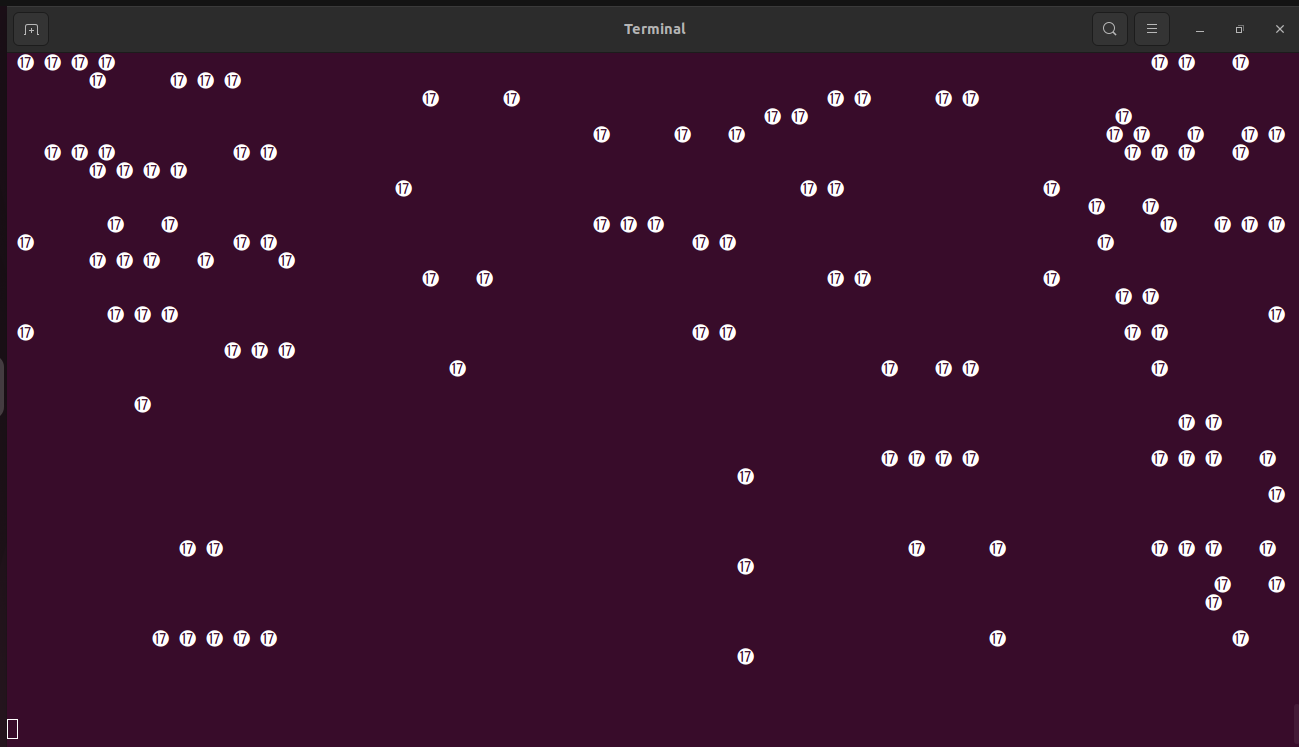
\includegraphics[width=120mm,scale=0.5]{figures/term.png}
    \captionof{figure}{Le jeu visible depuis le terminal}
\end{center}
\end{figure}


\subsection{Organisation du projet}

Dans un premier temps, la conception du logiciel à débuté avec une séance de brain-storming entre les membres du groupe sous la supervision du chargé de TP pour balancer les idées et propositions de chacun sur l'organisation du Projet

Différentes classes\ref{ref:les classes} :
Une fois d'accord sur les différentes classes nécessaires au développement du jeu, il était question de se repartir equitablement les tâches pour mener à bien le projet

Règles:
Certains membres du groupe étaient en charge de se renseigner sur les différents règles du jeu de la vie qui exsitent déjà et maîtiser les différences entre celles-ci.

Tests et Documentation :
L'intégration de tests unitaires pour assurer le bon fonctionnement des classes et des méthodes.

Pour la doc, la programmation par contrat nous a permis de générer automatiquement la Javadoc pour chaque classe et méthode du simulateur.

Outils collaboratifs :
Utilisation de GIT comme système de contrôle de version pour la modification des différents fichiers du simulateur.

Utilisation de Overleaf pour un suivi et accès du rapport et du PDF de la soutenance par toute l'équipe.

    \section{Elements techniques}

\subsection{Description des paquetages non standards utilisés}
    Paquetages non standards\label{ref:les classes} :

jeudelavie\textbf{.cellule :}  Contient toutes les classes concernées par les cellules du jeu.
jeudelavie\textbf{.grille :} Comprends les classes pour la gestion des grilles du jeu.
jeudelavie\textbf{.regles :} Contient les classes définissant les règles spécifiques du jeu.

jeudelavie\textbf{.interfacegraphique :} Comprend les classes pour l'interface graphique du jeu.

jeudelavie\textbf{.run :} Point d'entrée de l'application. Initialise l'interface graphique et démarre la simulation.

Pacquetages et classes principales :

Cellule.java : Représente une cellule individuelle du jeu, avec des méthodes pour gérer son état et ses voisins.

Grilles.java\label{exp} : Classe abstraite définissant les comportements communs des grilles de jeu.

Regles.java : Interface définissant les règles du jeu à implémenter pour différentes variantes.

Regle.java : Implémentation des règles de base du "Jeu de la Vie" selon Conway.
RegleHighLife.java : Implémentation des règles du "HighLife".
RegleDayAndNight.java : Implémentation des règles du "Day \& Night".

GrilleGUI.java : Fenêtre principale de l'interface graphique, affiche la grille et les contrôles (start, pause, reset).

\subsection{Description des algorithmes (non triviaux)}
Algorithme pour l'évolution des cellules :

\begin{algorithm}
  \SetAlgoLined
  \KwIn{Matrice $nbNecessaire$ représentant les configurations de voisins nécessaires, Entier $nbrCellV$ représentant le nombre de voisins vivants}
  \KwOut{État de la cellule (Vivant ou Mort)}
  
  \ForEach{ligne $row$ dans $nbNecessaire$}{
    \ForEach{élément $elem$ dans $row$}{
      \If{$elem == nbrCellV$}{
        \KwRet{Vivant}\;
      }
    }
  }
  \KwRet{Mort}\;
  
  \caption{Méthode de survie d'une cellule}
\end{algorithm}
Cet algorithme parcourt chaque cellule de la grille, compte les voisins vivants et détermine l'état de chaque cellule pour la prochaine génération en appliquant les règles spécifiques du Jeu de la Vie.\newline \newline

Algorithme des Voisins :\newline \newline \newline \newline \newline \newline \newline \newline 

\begin{algorithm}
  \SetAlgoLined
  \KwIn{Cellule $cell$}
  \KwOut{Nombre de voisins vivants}

  \SetKwArray{voisins}{voisins}
  \voisins $\gets$ tableau de 8 cellules contenant les voisins de $cell$\;
  
  \voisins[0] $\gets$ $cell$.getGrille().getCellule($cell$.getX() - 1, $cell$.getY() + 1)\;
  \voisins[1] $\gets$ $cell$.getGrille().getCellule($cell$.getX(), $cell$.getY() + 1)\;
  \voisins[2] $\gets$ $cell$.getGrille().getCellule($cell$.getX() + 1, $cell$.getY() + 1)\;
  \voisins[3] $\gets$ $cell$.getGrille().getCellule($cell$.getX() + 1, $cell$.getY())\;
  \voisins[4] $\gets$ $cell$.getGrille().getCellule($cell$.getX() + 1, $cell$.getY() - 1)\;
  \voisins[5] $\gets$ $cell$.getGrille().getCellule($cell$.getX(), $cell$.getY() - 1)\;
  \voisins[6] $\gets$ $cell$.getGrille().getCellule($cell$.getX() - 1, $cell$.getY() - 1)\;
  \voisins[7] $\gets$ $cell$.getGrille().getCellule($cell$.getX() - 1, $cell$.getY())\;

  $cpt \gets 0$\;
  \For{$c$ \textbf{in} \voisins}{
    \If{$c$.getArchiveEtat() $==$ Etat.Vivant}{
      $cpt \gets cpt + 1$\;
    }
  }
  
  \KwRet{$cpt$}\;

  \caption{Notre algorithme pour récupérer les voisins autour de chaque cellule}
\end{algorithm}


Algorithme pour générer des cellules aléatoirement : 
\lstinputlisting[language=Java,frame=single]{src.java}


\subsection{Description des structures de données (non triviales)}
    Comme structures de données que nous avons nous même dévéloppés, on peut citer: 
   \begin{enumerate}
       \item Grille : La classe Grilles représente la grille de cellules. Elle utilise un tableau de 2-dimensions pour stocker l'état de chaque cellule.
Propriétés :
lignes: Nombre de lignes dans la grille.
colonnes: Nombre de colonnes dans la grille.
listCelluleVivante: Liste des cellules vivantes dans la grille.

\item Cellule : La classe Cellule représente une cellule individuelle dans la grille.
Propriétés : x, y: Coordonnées de la cellule dans la grille.
etat: État actuel de la cellule (vivant ou mort).
etatArchive: État archivé de la cellule.
   \end{enumerate}
   



    \section{Architecture du projet: Diagrammes des modules et des classes}
Composants principaux :
\begin{enumerate}
    \item Cellule (Cellule.java) :
    \item Grille (Grilles.java) 
    \item Règles (Regle.java) 
    \item Interface Graphique :
    \item Structures de Données 
    \begin{enumerate}
        \item Enum Etat
    \end{enumerate} 

\end{enumerate}

\newpage
Voici sur la figure au dessus le diagramme de classe de notre projet, sur lequel figure les différents paquetages et ses interactions avec les autres paquetages.

    \begin{figure}
\begin{center}
        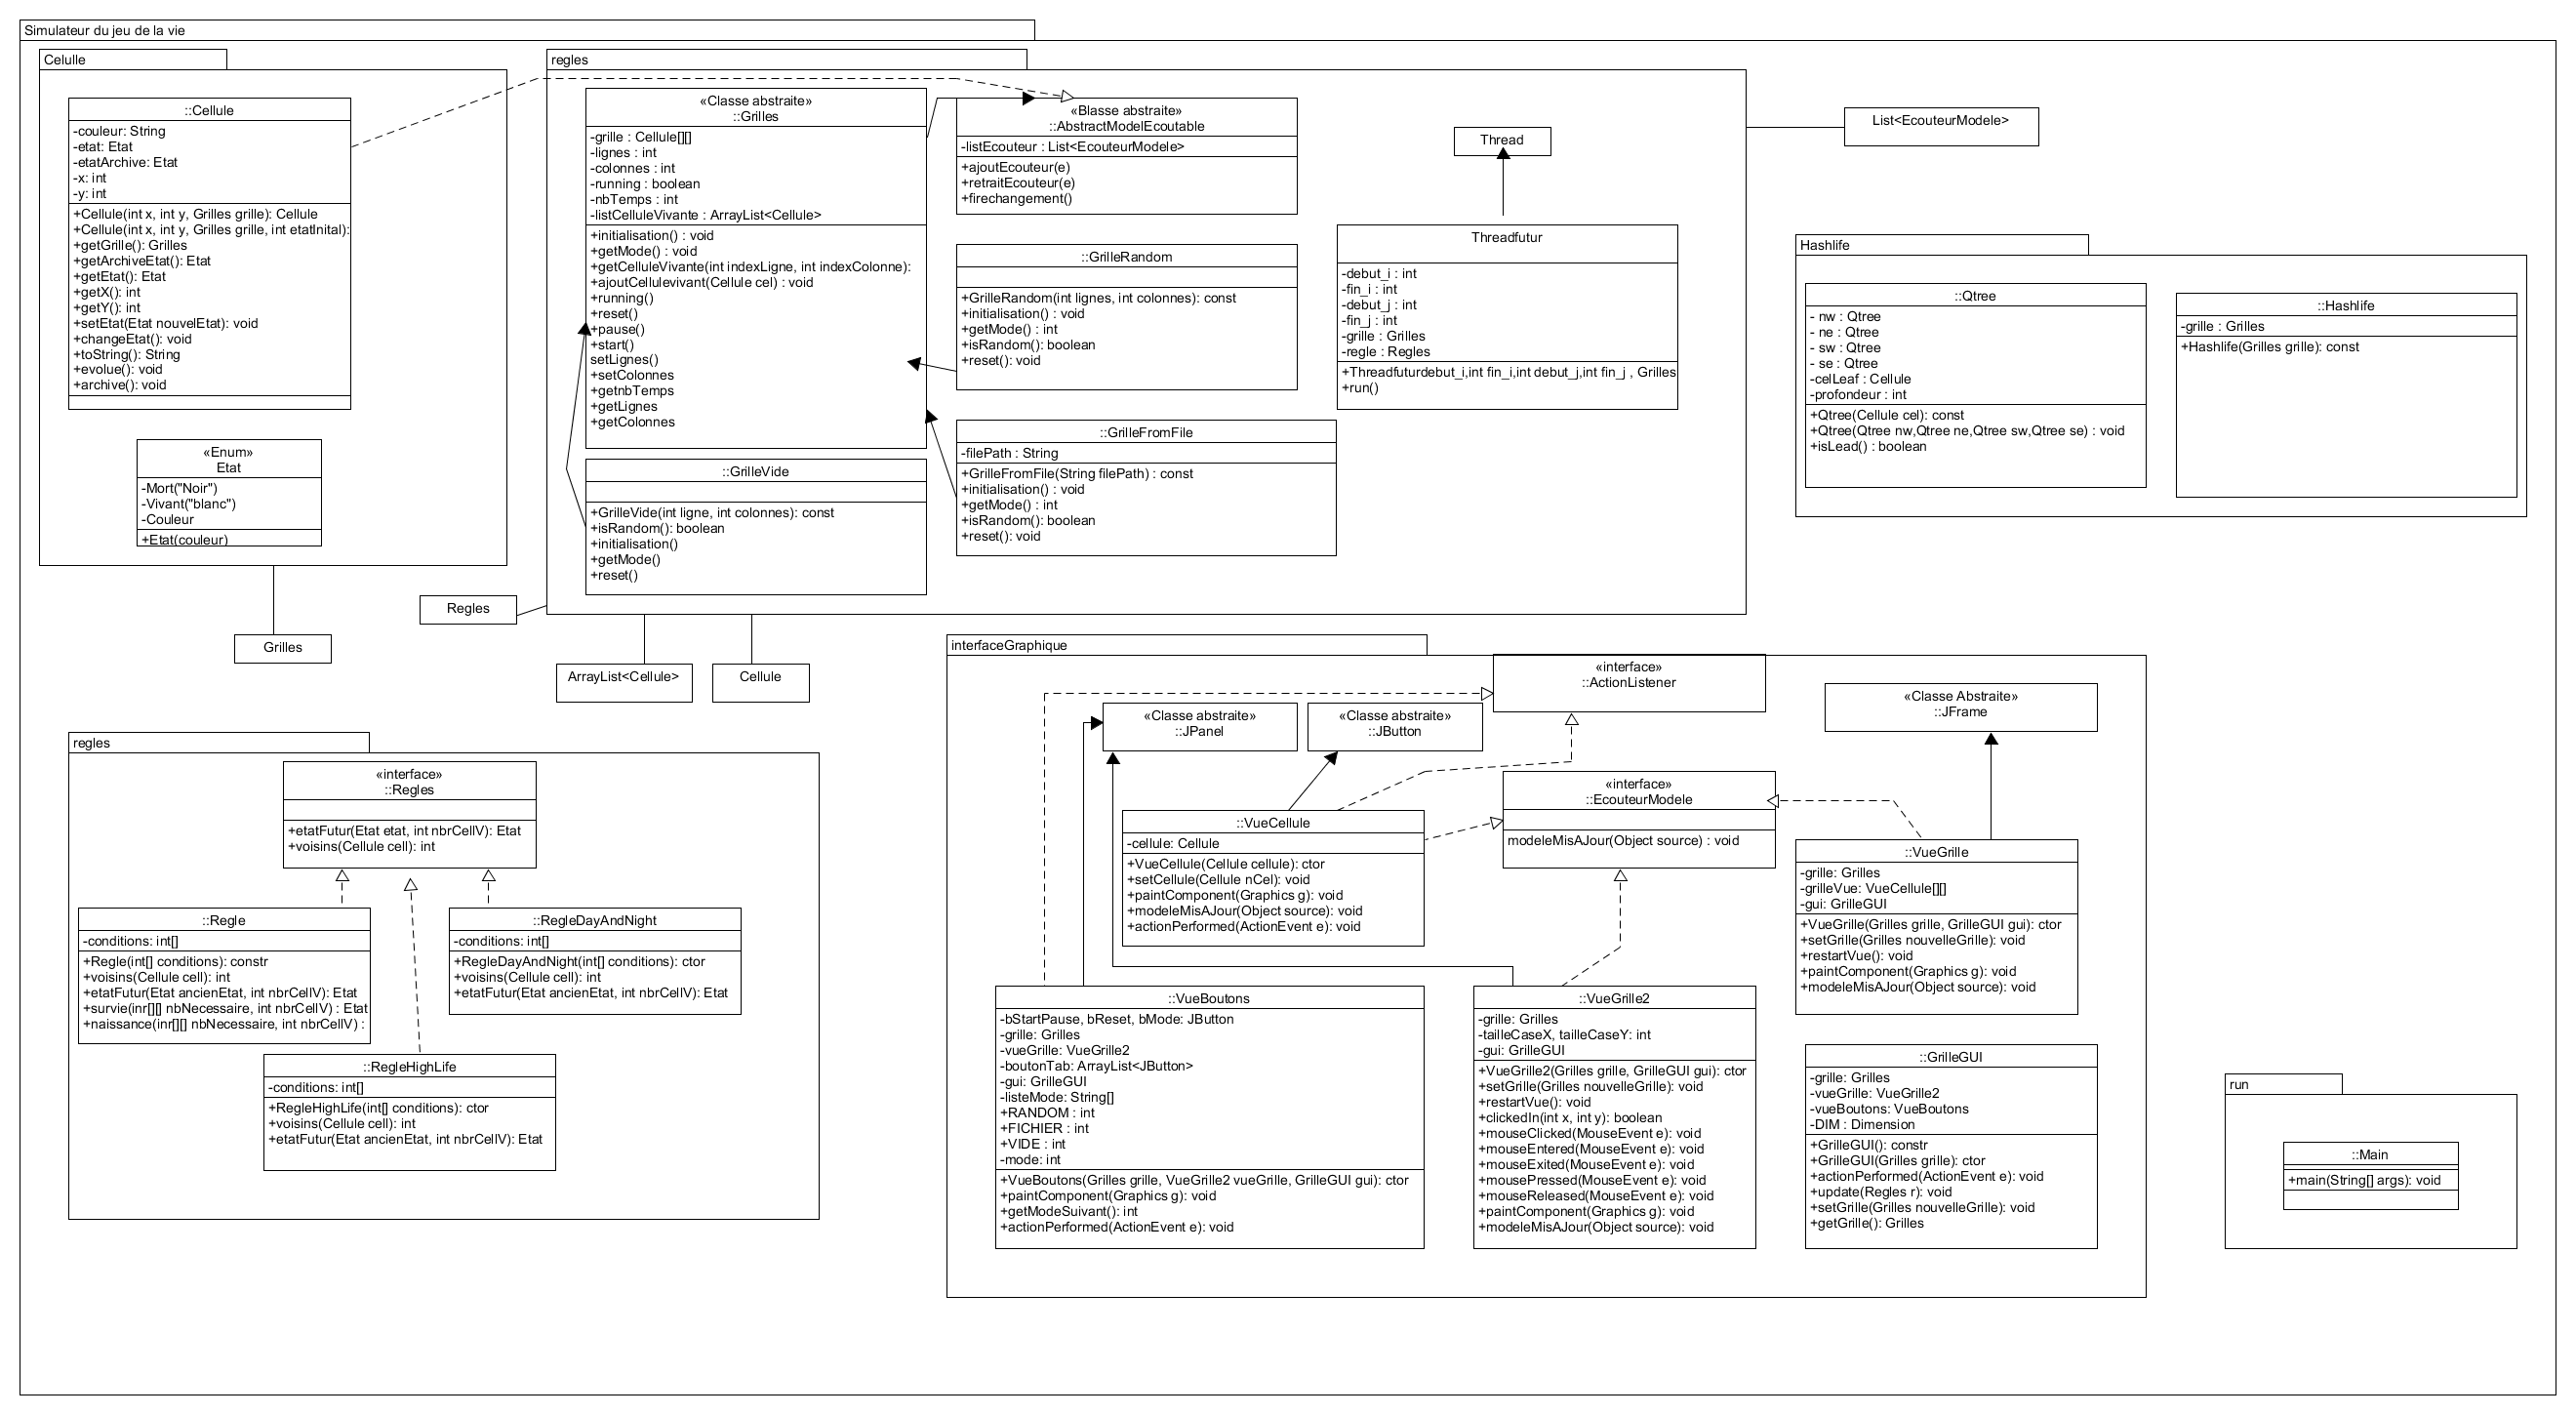
\includegraphics[width=120mm,scale=0.5]{figures/uml.png}
    \captionof{figure}{Diagramme de classe}
\end{center}
\end{figure}


\subsection{Chaînes de traitement (comment les classes interagissent et pourquoi)}

Interaction entre Grilles et Cellule :
Comme expliqué precedemment,\ref{exp} la classe Grilles représente la grille de cellules, tandis que la classe Cellule représente chaque cellule individuelle dans cette grille.
Pendant l'initialisation de la grille, Grilles crée un tableau 2D de Cellule pour représenter toutes les cellules de la grille.
Chaque cellule (Cellule) contient des informations sur son état (vivant ou mort via un Enum) et ses coordonnées (x et y).

Grilles utilise setEtat() pour modifier l'état d'une cellule en fonction des règles du jeu de la vie.

Interaction entre Regles et Grille:
La méthode futur(Regles r) de la classe Grilles est responsable de calculer l'état futur de chaque cellule en fonction des règles pré-definnies.

Pour chaque cellule dans la grille, Grilles utilise Regles.voisins() pour estimer d'abord le nombre de voisins vivants de la cellule puis avec cette info, Grilles utilise ensuite Regles.etatFutur() pour fixer le nouvel état de la cellule (vivant ou mort) à la prochaine génération.


Interaction partie graphique :

Les classes VueGrille et VueGrille2 sont responsables de l'affichage graphique de la grille de cellules.
Elles reçoivent des mises à jour de la grille à partir de modeleMisAJour(Object source) quand y a des changements
Ces vues parcourent le tableau de Cellule pour afficher avec l'itrface graphiqu chaque cellule à l'écran, en utilisant leurs états (Etat.Vivant ou Etat.Mort) pour déterminer la couleur.

Interaction avec l'interface utilisateur (GrilleGUI) :

La classe GrilleGUI agit comme une interface utilisateur pour le jeu.
Elle utilise (VueGrille, VueBoutons) pour afficher la grille et permettre à l'utilisateur d'interagir avec le jeu (start, pause, réinitialiser).
Lorsque l'utilisateur cliques sur les boutons ("Start" ou "Reset"), des événements (ActionEvent) sont lancés, ce qui conduit à des actions comme démarrer ou arrêter la simulation dans la grille (Grilles).

    \section{ Expérimentations et usages}
\subsection{Interface graphique:}


pour l'interface graphique on a decidé de separé en deux JPanel le Jframe l'un qui affichera la grille en l'etat et son nombre de tour effectué et l'autre JPanel qui servira de controleur avec trois boutons pour soit commencé ou mettre en pause la simultation un bouton Reset qui fait recommencé la simulation a zero ou genere un autre grille pour la grille aleatoire et un dernier bouton qui permet de changer le mode de la grille (fichier , aleatoir,vide) 
on avait aussi voulu implement un dernier bouton qui aller lui changer le mode de regle disponible

Pour ce qui est du Jpanel de la grille on a deux options soit affiché la grille avec des Jbutton ce qui rend la classe VueGrille tres lourdes car pour chaque cellule elle crée une nouvelle class VueCelulle qui utilise le jbutton , l'aventage de cette classe JPanel est qu'elle évite de devoir implementer l'interface MouseListener pour le clique sur le changement de cellule mais en termes de vitesse d'execution la deuxième classe VueGrilleÉ est bien meilleur.
Non seulement VUeGrille2 utilise la classe JscrollPane qui permet d'avoir une grille d'une taille superieur à 300x300.La classe utilise dans la méthode paintComponent() la méthode getCelluleVivante() de la classe abstraite Grilles qui permet d"eviter de faire des test pour chaque case de la grille et donc de verifier à chaque fois si la case doit être desciner ou non .  



\subsection{Cas d’utilisation (exemples d’utilisation avec capture d’écran)}
Démarrer la simulation :

Capture d'écran :

Étapes :
L'utilisateur ouvre l'application .
La grille de cellules est initialisée avec un état aléatoire ou vide.
L'utilisateur appuie sur le bouton "Start" pour démarrer la simulation.
Les cellules évoluent en fonction des règles de Conway.

Interaction UI\footnote{User interface => interface utilisateur}  :
L'utilisateur peut directement cliquer sur la grille et les cellules pour les faire naître ou mourir.

Capture d'écran :

Étapes :
L'utilisateur utilise la souris pour cliquer sur une cellule.
Si la cellule est vivante, elle meurt et devient noire.
Si la cellule est morte, elle naît et devient blanche.


Cas d'utilisation : Arrêter le jeu

L'utilisateur arrête la simulation en cours et réinitialise la grille.

Capture d'écran :

Étapes :
L'utilisateur appuie sur le bouton "Pause" pour arrêter la simulation.
L'utilisateur appuie sur le bouton "Reset" pour réinitialiser la grille à son état initial.
\newpage

    \section{Conclusions}
\label{ch:con}
\subsection{Récapitulatif des fonctionnalités principales}
Pour résumer, comme vous l'aurez remarqué, le jeu de la vie n'est pas un jeu à proprement dit: notre projet combine les concepts du jeu de la vie de Conway avec une interface graphique Java(swing) pour offrir une expérience interactive, digne des meilleurs simulateurs du jeu de la vie sur le net. 
Les fonctionnalités majeures incluent la simulation automatisée des règles du jeu, la possibilité d'interaction directe avec la grille et une interface utilisateur simple mais efficace pour contrôler la simulation, sans oublier que le jeu est directement jouable depuis le terminal.

L'objectif principal était de fournir une implémentation visuellement attrayante du jeu de la vie, donnant possibilité à l'utilisateur de découvrir les principes de l'automate cellulaire de Conway.


\subsection{Propositions d’améliorations}
Déjà, ce qui à été fait: 
La grille affiche un état initial aléatoire, chargé ou vide.
Les règles de Conway sont appliquées pour faire évoluer les cellules.
L'utilisateur peut démarrer, mettre en pause et réinitialiser la simulation.

Interaction Utilisateur :
L'utilisateur peut cliquer sur les cellules pour les faire naître ou mourir.
Les cellules vivantes sont représentées en blanc et les cellules mortes en noir.
Interface Graphique :
L'interface utilise Swing pour créer une fenêtre graphique conviviale.
Des boutons permettent de contrôler la simulation (démarrer, mettre en pause, réinitialiser).
Mise à Jour Dynamique :
La vue de la grille est mise à jour dynamiquement à chaque étape de simulation.
Les changements d'état des cellules sont reflétés graphiquement en temps réel.

    Pour améliorer le simulateur du jeux de la vie, quelques améliorations peuvent être apportés:
    \begin{itemize}
        \item Permettre à l'tilisateur de choisir la taille de sa grille
        \item Permettre à l'utilisateur de choisir les couleurs des cellules mortes ou vivantes
        \item Choisir la règle depuis une liste déroulante
        \item Trouver une solution pour la bar de scroll
        \item Faire fonctionner le HashLife
    \end{itemize}
    

    \bibliographystyle{unsrt} 
    
    \section*{References}
    \begin{itemize}
   \item\href{http://pdbzro.com/gags/math/jeudelavie.pdf}{Jeu de la vie}
    \item\href{https://conwaylife.com/wiki/Main_Page}{Lifewiki}
    \item\href{https://neuralpatterns.io/}{Automates Cellulaires neureux}
    \item\href{https://www.youtube.com/watch?v=S-W0NX97DB0}{Science Etonnante : jeu de la vie}
    \end{itemize}
    
    
\end{document}
